\subsection{Integration in die UH Codebase}
\subsubsection{Das Kartenformat}
\label{kartenformat}

%
% algorithm principle
%
\begin{figure}[htbp]
  \centering
  
    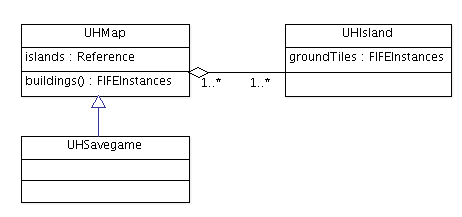
\includegraphics[width=0.7\textwidth]{gfx/klassendiagramm-UHSaveGame.png}
  
  \caption{UML Diagramm des Kartenformates von UH.}
  \label{figure:automaton-intersection}
\end{figure}

UHs Kartenformat in SQLite besteht grob aus den folgenden Elementen für den
Editor relevanten Elementen:
\begin{itemize}
  \item Allgemeinen Karteninformationen
  \item Die auf der Karte plazierten Objekte (wie Gebäude etc.)
  \item Verweise auf Island-Files. \\ 
  Ein Island-File ist eine SQLite-Datenbank,
  die die Informationen über die Bodenbeschaffenheit einer zusammengehörenden
  Inseln enthält:
  \begin{itemize}
    \item Allgemeine Islandinformationen
    \item Alle zu einem Island gehörenden Groundtiles
  \end{itemize}
\end{itemize} 

\subsection{Kommandozeilen-Parameter (FIFE)}
\subsection{Schaffung der Plugin-Infrastruktur (FIFE)}

\subsection{Plugin zum Laden von UH Objekten (UH)}
UH speichert alle dem Spiel zur Verfügung stehenden Objekte in mehreren Dateien
und Verzeichnissen:

\begin{description}
\item[content/objects] Dieser Ordner enthält mehrere Unterordner, die wiederum
YAML-Dateien\footnote{Ein Dateiformat, siehe \cite{yaml}} enthalten. Jede
dieser Dateien definiert ein Objekt und seine zugehörigen Eigenschaften.
\item[content/gfx] Dieser Ordner enthält die Grafiken, die zu den Objekten
gehören. Dabei sind die Grafiken für animierte Objekte auf mehrere Dateien
aufgeteilt, die in sogenannte ActionSets gruppiert werden.
\end{description}

UH bietet Klassen an, um diese Daten einzulesen und sie dem Editor
verfügbar zu machen. Mithilfe dieser Klassen war es uns möglich, ein
Plugin für den FIFE Editor zu erstellen, das alle Gebäude und Bodentiles
laden und dem Editor zur Verfügung stellen kann.

Das Plugin besteht aus einer einzigen Klasse: \code{UHObjectLoader}. Diese
Klasse wird vom Editor geladen und anschließend wird ihre \code{enable()} Methode
aufgerufen. Diese lädt anschließend erst alle Groundtiles und dann alle Gebäude.
Sobald die Objekte der Engine bekannt sind, können diese mittels der vom Editor
bereitgestellten Werkzeuge auf Maps platziert werden.

\subsubsection{Groundtiles}
Um die Groundtiles zu laden wird die UH-Klasse \code{GroundTileLoader} benutzt,
die alle vorhandenen Groundtiles einliest und als Liste zurückgibt. Anschließend
wird für jedes der Tiles ein \code{Object} und ein \code{InstanceVisual} in der
Engine erstellt, sowie mehrere \code{Action}s und \code{ActionVisual}s, um Animationen darzustellen.
Alle diese Objekte benötigt die Engine, um die Tiles später im Editor korrekt
darstellen zu können.

\subsubsection{Gebäude}
Für die Gebäude müssen zunächst die XML-Deskriptoren ausgelesen werden, die
zusätzliche Informationen zu jedem Gebäude enthalten, wie z.B. dessen Größe.

Anschließend werden wiederum ein \code{Object}, \code{InstanceVisual} und
mehrere \code{Action}s und \code{ActionVisual}s erstellt, um das Gebäude in
der Engine zu registrieren.


\subsection{Plugin zum Laden von UH Karten (UH)}
\subsection{Plugin zum Speichern von UH Karten (UH)}
Das Plugin zum Speichern weist die Schwierigkeit auf, dass der Editor nicht die
Interna des UH Spielmodells kennen kann. Der Editor ``zeichnet'' einfach nur
Elemente wie Bodentiles und Gebäude auf die verschiedenen Layer-Schichten, das
Saver-Plugin muss diese im UH-Modell speichern. 


Die Layer-Schichten enthalten vor dem Speichern die Instanzen aller vom User
gesetzen Gebäude und Bodentiles. 

Der Algorithmus geht dabei den Groundlayer vom Urpsrung des Koordinatensystems
Origo (0, 0) nach rechts unten ab. Durch diese Traversierungsstrategie muss nur
nach oben und nach links auf zu verbindenden Islands überprüft werden. Findet
sich ein direkt angrenzendes Groundtiles, so wird das akutelle Groundtiles (rot
hinterlegt) mit dem bestehenden vereinigt, indem es dessen Insel-ID übernimmt.

%
% algorithm principle
%
\begin{figure}[htbp]
  \centering
  
    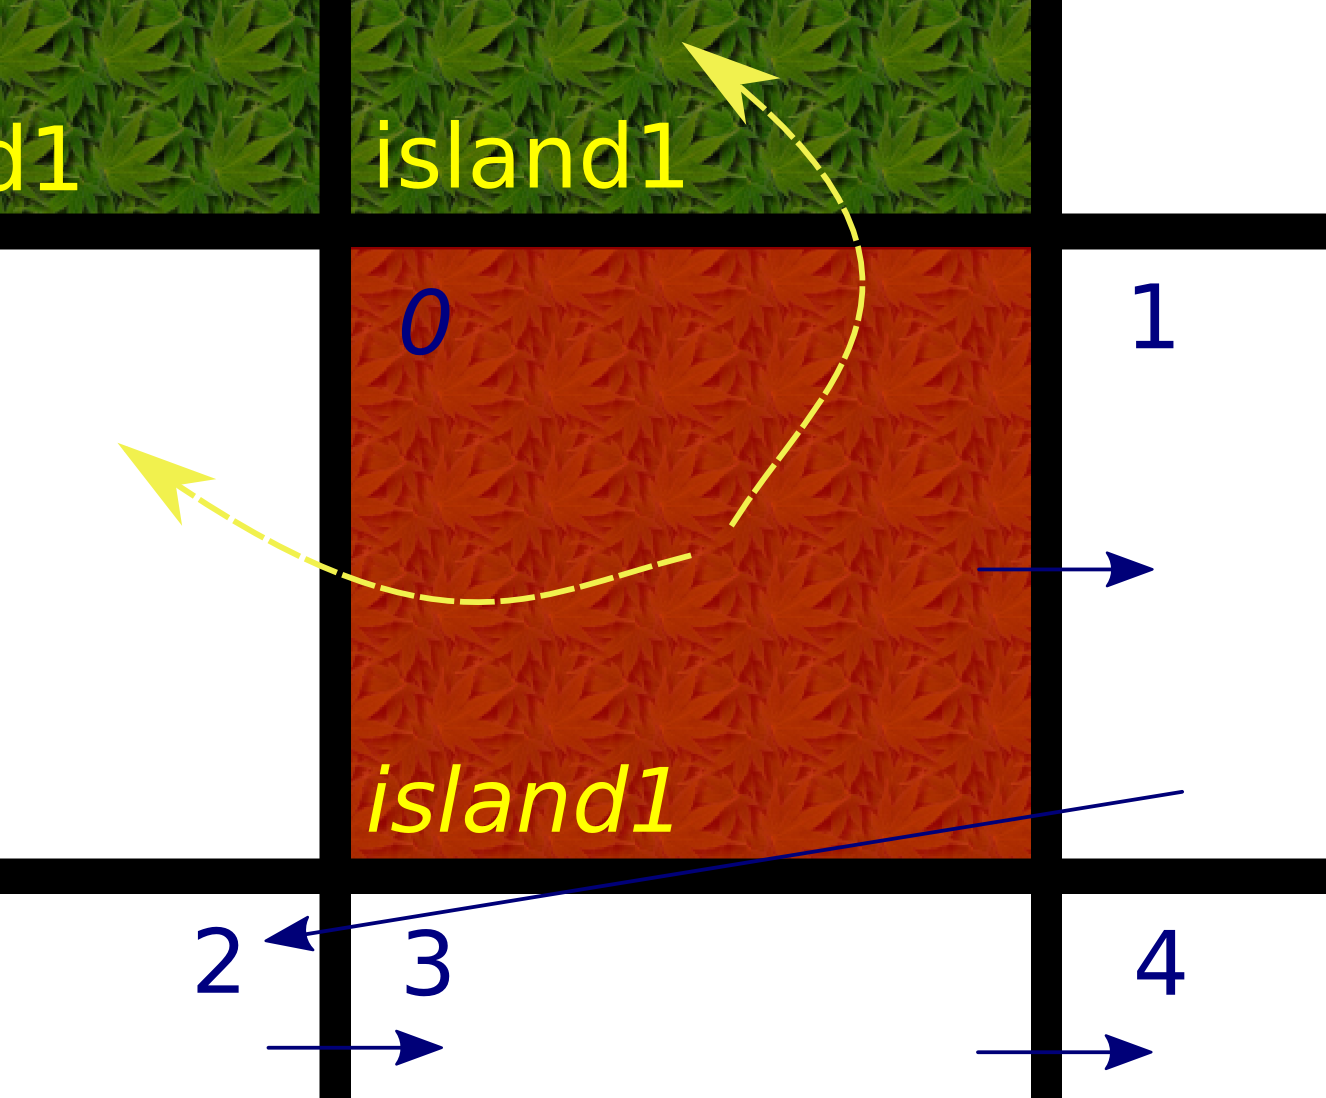
\includegraphics[width=0.7\textwidth]{gfx/merge_algorithm.png}
  
  \caption{Der Partitionierungsalgorithmus für die Islands. Die gelben Pfeile
  geben an, welche Gitterflächen auf das Vorhandensein von Tiles überprüft
  werden. Der Algorithmus traversiert die Tiles von oben links nach unten
  rechts (blau eingezeichnet).}
  \label{figure:automaton-intersection}
\end{figure}

Wie in Abschnitt \ref{kartenformat} erklärt, besteht die Schwierigkeit des
Transformationsprozesses in diese Richtung darin, zusammenliegende Bodentiles zu
erkennen. Dadurch benötigt das Speichern großer Inseln eine gewisse Zeit bis die
Gruppierung der Inslen beendet ist.
